%!TEX root=../main.tex

\section{Introduction}\label{sec:intro}

%The goal of this work is to make optimization for two-layer neural networks a reliable technology.
%A technology is robust and consistent, comes with guarantees, and can be employed without specialist knowledge.
%Despite their popularity, current methods for training neural networks fail at these criteria.
%For researchers, the result has been a fantastic proliferation of new ideas as the machine learning community explores non-convex optimization.
%For practitioners, however, the outcome is a crowded field of competing algorithms.

\begin{figure}[t]
	\centering
	\ifdefined\smallPDF
		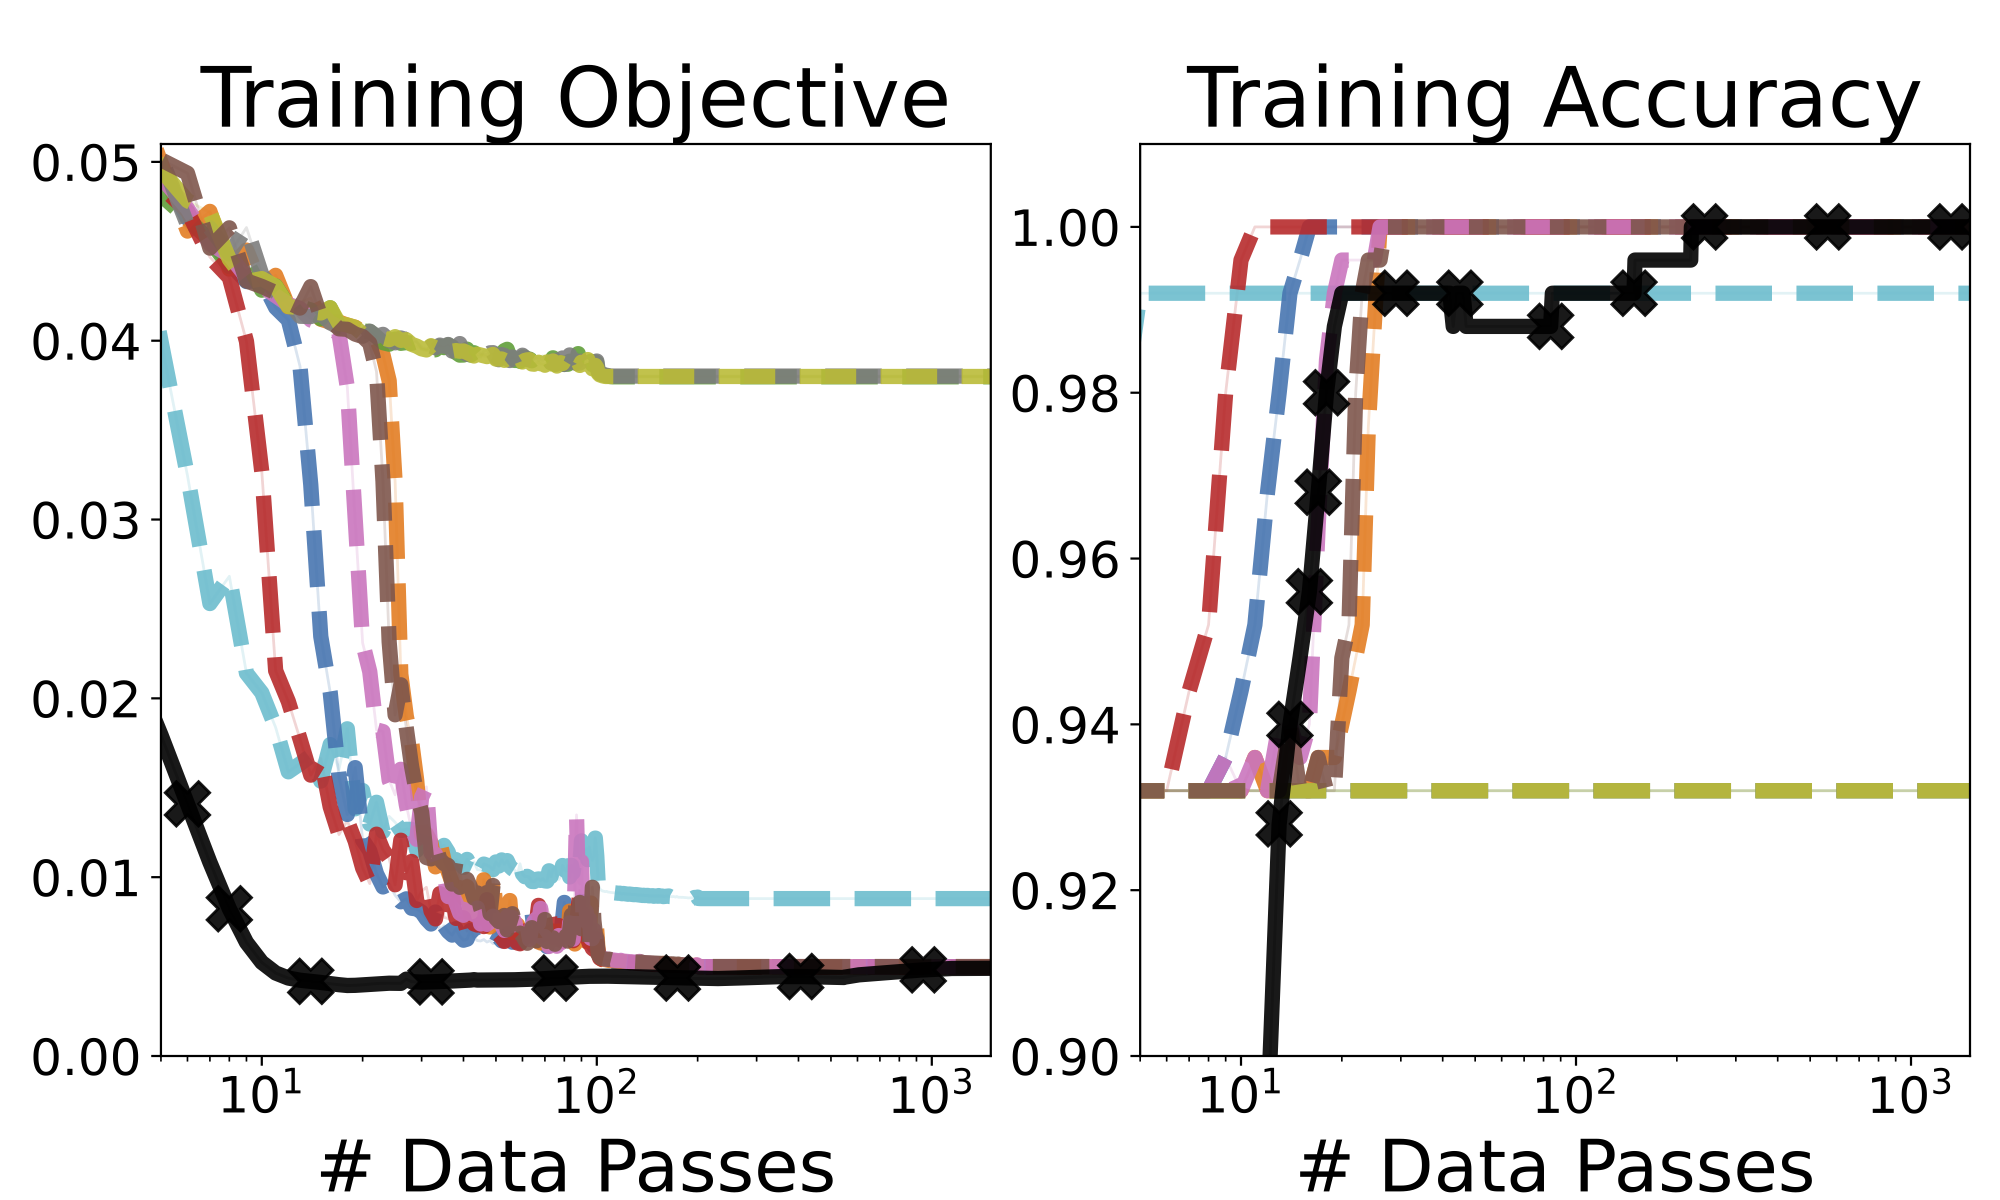
\includegraphics[width=\linewidth]{figures/chapter_two/synthetic_classification.png}
	\else
		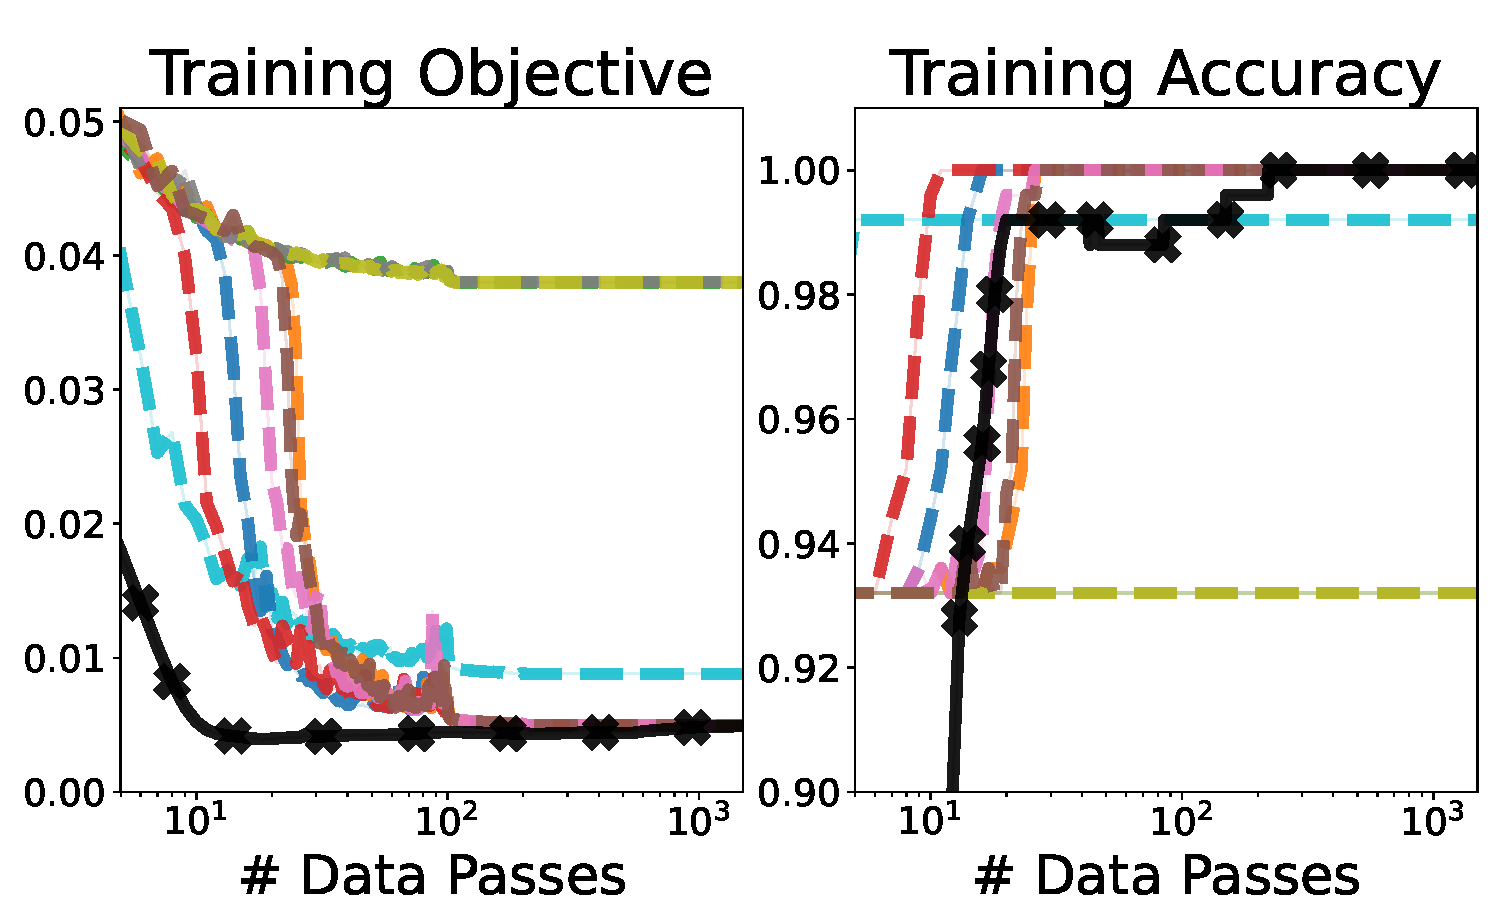
\includegraphics[width=\linewidth]{figures/chapter_two/synthetic_classification.pdf}
	\fi
	\vspace{-1.5em}
	\caption{Convex (solid line) and non-convex (dashed) optimization of a two-layer ReLU network for a realizable synthetic classification problem.
		We plot only one run of the convex solver since they are nearly identical and all reach perfect accuracy.
		In contrast, \( 4/10 \) runs of SGD on the non-convex problem converge to sub-optimal stationary points.
	}%
	\label{fig:synthetic-classification}
	\vspace{-0.5cm}
\end{figure}

It is well-known that global optimization of neural networks is NP-Hard~\citep{blum1988npcomplete}.
Despite the theoretical difficulty, highly accurate models are trained in practice using stochastic gradient methods (SGMs)~\citep{bengio2012practical}.
Unfortunately, SGMs cannot guarantee convergence to a local optimum of the non-convex training loss~\citep{ge2015escaping} and existing methods rarely certify convergence to a stationary point of any type~\citep{goodfellow2016deeplearning}.
SGMs are also sensitive to hyper-parameters;
they converge slowly, to different stationary points~\citep{neyshabur2017implicit}, or even diverge depending on the choice of step-size.
Parameters like the random seed complicate replications and can produce model churn, where networks learned using the same procedure give different predictions for the same inputs~\citep{henderson2018deep, bhojanapalli2021reproducibility}.
See \autoref{fig:synthetic-classification} for an example.
For most applications, practitioners use domain knowledge and costly hyper-parameter search to cope with these challenges.

In contrast, we propose to optimize shallow models via \emph{convex reformulations} of the training objective.
Recent work by \citet{pilanci2020convexnn} uses duality theory to show two-layer neural networks with ReLU activations and weight decay regularization may be re-expressed as a linear model with a group-$\ell_1$ penalty and polyhedral cone constraints.
Subsequent research extends this model space, deriving convex formulations for convolutions~\citep{sahiner2020convex,ergen2021implicit,gupta2021exact}, vector-outputs~\citep{sahiner2021vector}, batch normalization \cite{ergen2021demystifying}, generative models \cite{sahiner2021hidden} and deeper networks~\citep{ergen2021beyond, ergen2021revealing}.
However, existing work is largely focused on model classes, rather than leveraging convexification to train neural networks.

This paper develops fast optimization algorithms for two-layer ReLU models by carefully studying the space of equivalent models.
We show that unregularized ReLU networks can be trained by decomposing the solution to an unconstrained generalized linear model (GLM) onto a difference of polyhedral cones.
With non-zero regularization, the same unconstrained problem yields a data-dependent approximation of the optimal solution which differs only in the norm of the model weights.
To fit this GLM, we develop a proximal-gradient method that combines the convex optimization toolbox with GPU acceleration.
We also use this optimizer as a sub-routine for an augmented Lagrangian method that quickly and robustly trains ReLU networks via the (constrained) convex reformulation.
Our deterministic optimizers give both convergence and optimality guarantees.

To summarize, our main contributions are the following:
\begin{itemize}
	\item A new class of \emph{unconstrained} convex optimization problems which are equivalent to training an unregularized ReLU model and approximation guarantees for the case of non-zero regularization.

	\item An accelerated proximal-gradient method for this unconstrained problem that improves the complexity of computing a global optimum from \(O(1/\epsilon^2)\) to \(O(1/\sqrt{\epsilon})\) iterations compared to subgradient methods.

	\item An augmented Lagrangian method for the constrained convex reformulation which uses our unconstrained solver as a sub-routine and outperforms commercial interior-point software such as MOSEK~\citep{mosek}.

	\item Extensive experiments which validate our theoretical results, carefully explore the properties of our optimization methods, and scale convex optimization for ReLU networks to MNIST and CIFAR-10.
\end{itemize}

Quality software is key to practical use of our methods.
As such, we also provide \texttt{scnn}, an open-source package for training neural networks by convex optimization.\footnote{\small \url{https://github.com/pilancilab/scnn}}

\subsection{Related Work}

Our work combines ideas from the literature on convex neural networks, accelerated methods, and constrained solvers.

\textbf{Convex Neural Networks}:
%In addition to the theory based on semi-infinite duality, other attempts have been made to relate neural networks with convexity.
There have been repeated attempts to develop convex neural networks.
\citet{bengio2006convex} view two-layer neural networks as convex models, but their work requires the first-layer weights to be fixed.
Similarly, extreme learning machines \citep{huang2005elm} obtain a convex problem by using a random first-layer;
these models can obtain zero training error for over-parameterized problems
\citep{woodworth2020rich}, but do not learn parsimonious latent representations as in our approach.

\citet{bach2017breaking} analyze infinite-width two-layer networks; these methods are not implementable, but may be viewed as convex problems.
Other research considers the separate problem of neural networks for which the prediction function is convex~\citep{amos2017input, sivaprasad2021curious}.

In concurrent work, \citet{bai2022efficient} consider training two-layer
ReLU networks via convex reformulations using ADMM.
Their approach requires solving a linear system at each iteration,
or uses coordinate descent to solve the ADMM sub-problems.
In practice, our solvers scale to larger datasets
and allow for more activation patterns.

\textbf{Accelerated Proximal Gradient}:
\citet{beck2009fista, nesterov2007proximalgradient} were the first to extend optimal gradient methods~\citep{nesterov1983method} to composite problems.
Work since then includes extensions to stochastic~\citep{schmidt2011convergence} and non-convex~\citep{li2015accelerated} optimization.
See~\citet{parikh2014proximalsurvery} for a survey of proximal algorithms, including proximal gradient.

\textbf{Augmented Lagrangian Methods}: The convergence theory was initially developed by Rockafellar~\citep{rockafellar1976augmented, rockafellar1976monotone}.
More recent work includes practical guidelines~\citep{birgin2014pratical} and acceleration techniques~\citep{kang2015inexact}.
See \citet{bertsekas2014constrained} for exhaustive theoretical developments.

